\documentclass{ut-thesis}

% Administrative data only.  Thesis prose belongs in chapters/ and appendices/.
\thesissetup{
  university-fa={دانشگاه تهران},
  college-fa={دانشکدگان فنی},
  faculty-fa={دانشکده برق و کامپیوتر},
  degree-fa={کارشناسی ارشد},
  subject-fa={مهندسی فناوری اطلاعات},
  field-fa={},
  title-fa={عنوان نمونه پایان‌نامه},
  author-fa={نام و نام خانوادگی},
  student-id={شماره دانشجویی},
  date-fa={ماه و سال},
  supervisor-fa={نام و مشخصات},
  supervisor-rank-fa={},
  advisor-one-fa={نام و مشخصات},
  advisor-two-fa={نام و مشخصات},
  advisor-one-rank-fa={},
  advisor-two-rank-fa={},
  advisor-one-affiliation-fa={},
  advisor-two-affiliation-fa={},
  internal-judge-fa={نام و مشخصات},
  internal-judge-rank-fa={},
  external-judge-fa={نام و مشخصات},
  external-judge-rank-fa={},
  graduate-deputy-fa={نام و مشخصات},
  graduate-deputy-rank-fa={},
  keywords-fa={قالب، نگارش، نمونه},
  university-en={University of Tehran},
  college-en={College of Engineering},
  faculty-en={School of Electrical and Computer Engineering},
  degree-en={Master of Science},
  subject-en={Information Technology Engineering},
  field-en={},
  title-en={A Sample Thesis Title},
  author-en={Student Name},
  date-en={Month Year},
  supervisor-en={Advisor Name},
  advisor-one-en={Advisor Name},
  advisor-two-en={Advisor Name},
  keywords-en={Template; Writing; Example},
  include-besm=true,
  include-defense=true,
  include-originality=true,
  include-ai-report=true,
  include-dedication=true,
  include-acknowledgements=true,
  include-list-of-tables=true,
  include-list-of-figures=true,
  include-english-pages=true
}

\addbibresource{bibliography/references.bib}
% Define paired semantic terms here; registry is refreshed before each build.
\newglossaryentry{dataset}{type=faen,name={مجموعه داده},text={مجموعه داده},
 first={\ThesisTermFirst{مجموعه داده}{dataset}},description={dataset}}
\newglossaryentry{en-dataset}{type=enfa,name={dataset},description={مجموعه داده}}
\newglossaryentry{user-interface}{type=faen,name={رابط کاربری},text={رابط کاربری},
 first={\ThesisTermFirst{رابط کاربری}{user interface}},description={user interface}}
\newglossaryentry{en-user-interface}{type=enfa,name={user interface},description={رابط کاربری}}
\newacronym[user1={رابط کاربری}]{acr-user-interface}{UI}{user interface}
% Deliberately unused: must not appear in generated lists.
\newglossaryentry{unused-term}{type=faen,name={اصطلاح استفاده‌نشده},description={unused term}}
\newglossaryentry{en-unused-term}{type=enfa,name={unused term},description={اصطلاح استفاده‌نشده}}


\begin{document}

% Preliminary pages: deliberately no automatic blank versos.
\pagestyle{empty}
\pagenumbering{gobble}
\ThesisPersianCoverPage
\ifThesisIncludeBesm\ThesisBesmPage\fi
\ThesisPersianTitlePage
\ifThesisIncludeDefense\ThesisDefenseCertificatePage\fi
\ifThesisIncludeOriginality\ThesisOriginalityPage\fi
\ifThesisIncludeAIReport
  \ThesisContentPage{گزارش استفاده از هوش‌مصنوعی}{front-matter/ai-use-disclosure.tex}
\fi
\ifThesisIncludeDedication
  \ThesisContentPage{تقدیم}{front-matter/dedication-text.tex}

\fi
\ifThesisIncludeAcknowledgements
  \ThesisContentPage{سپاسگزاری}{front-matter/acknowledgements-text.tex}

\fi
\ThesisPersianAbstractPage

% Persian alphabetic folios for the preliminary lists.
\clearpage
\thesisstartlistpages
\pagestyle{thesisfront}
\tableofcontents
% Generated by tools/prepare_terms.py; edit glossary/terms.tex instead.
\glsadd{acr-user-interface}
\glsadd{en-dataset}
\glsadd{en-user-interface}

\printnoidxglossary[type=\acronymtype,title={فهرست علائم، نشانه‌ها و مخفف‌ها},style=thesisacronyms]
\ifThesisIncludeTables
  \ThesisListOfTables
\fi
\ifThesisIncludeFigures
  \ThesisListOfFigures
\fi

% Main body.
\clearpage
\pagenumbering{arabic}
\pagestyle{thesismain}
\chapter{مقدمه}\label{ch:introduction}
\section{هدف و ساختار نوشته}
این پایان‌نامه نمونه، شیوه استفاده از قالب را نشان می‌دهد. همه متن‌ها آموزشی هستند و باید با نوشته نویسنده جایگزین شوند. برای آشنایی با نگارش ساختاریافته به منبع \cite{lamport1994} مراجعه کنید.

یک \gls{dataset} در این مثال تنها چند مقدار ساختگی دارد. استفاده دوباره از \gls{dataset} نباید پاورقی انگلیسی تازه‌ای بسازد. عبارت \lr{sample.txt} و عدد \thesisnum{۱۲٫۵} نمونه‌ای از ترکیب متن فارسی و لاتین هستند.
\section{راهنمای خواندن}
فصل \ref{ch:method} روش نمونه و شکل \ref{fig:workflow} مراحل آن را نشان می‌دهد. واژه‌های \textbf{پررنگ} و \emph{تأکیدی} نیز قابل استفاده‌اند.
\begin{itemize}
\item هر فصل در پرونده‌ای مستقل نوشته می‌شود.
\item ارجاع‌ها با کلید معنایی نگهداری می‌شوند.
\end{itemize}

\chapter{پیشینه و مبانی}
این بخش نمونه‌ای از مقدمه بدون شماره بخش است.
\section{نگارش علمی}
ساختار منطقی سند از ظاهر آن جدا نگه داشته می‌شود \cite{knuth1984,lamport1994}. عنوان‌ها در فهرست مطالب و نشانک‌های فایل خروجی قابل دسترسی هستند.
\subsection{اصطلاحات}
یک \gls{user-interface} باید خوانا باشد. کلید اصطلاح را در واژه‌نامه تعریف کنید و در متن به همان کلید ارجاع دهید.

\chapter{روش پژوهش}\label{ch:method}
در این نمونه، سه مرحله برای نمایش یک فرایند ساده در نظر گرفته شده است.
\section{مراحل کار}
\begin{figure}
\centering
\begin{tikzpicture}[every node/.style={draw,rounded corners,minimum width=28mm,minimum height=12mm}]
\node (a) at (0,0) {\rl{ورودی}};
\node (b) at (4,0) {\rl{پردازش}};
\node (c) at (8,0) {\rl{خروجی}};
\draw[->,thick] (a)--(b);\draw[->,thick] (b)--(c);
\end{tikzpicture}

\caption[مراحل نمونه]{مراحل نمونه شامل دریافت ورودی، پردازش و بررسی خروجی است. این توضیح بلند فقط زیر شکل نمایش داده می‌شود.}
\label{fig:workflow}
\end{figure}
\section{تعریف کمیت}
میانگین مقادیر با رابطه \ref{eq:mean} تعریف می‌شود.
\begin{equation}\label{eq:mean}
\bar{x}=\frac{1}{n}\sum_{i=1}^{n}x_i
\end{equation}

\chapter{پیاده‌سازی نمونه}
در این فصل، نحوه نمایش اطلاعات ساختاریافته بررسی می‌شود.
\section{جدول}
\begin{table}[ht]
\centering
\caption[پارامترهای نمونه]{پارامترهای ساختگی برای نمایش جدول؛ این مقادیر نتیجه آزمایش واقعی نیستند.}\label{tab:parameters}
\begin{tabular}{rr}\toprule
پارامتر & مقدار\\\midrule
تعداد مرحله & \thesisnum{۳}\\
اندازه نمونه & \thesisnum{۱۰}\\\bottomrule
\end{tabular}
\begin{ThesisTableNotes}یادداشت جدول: واحدها را در عنوان ستون مشخص کنید.\end{ThesisTableNotes}
\end{table}
\section{فهرست ترتیبی}
\begin{enumerate}\item ورودی را بررسی کنید.\item خروجی را ثبت کنید.\end{enumerate}

\chapter{نمایش نتایج نمونه}
اعداد این فصل ساختگی‌اند و تنها برای آموزش درج نمودار آمده‌اند.
\section{نمودار}
\begin{ThesisChart}
\centering
% Synthetic demonstration values only; heights are in centimetres.
\def\SampleA{2}\def\SampleB{3}\def\SampleC{4}

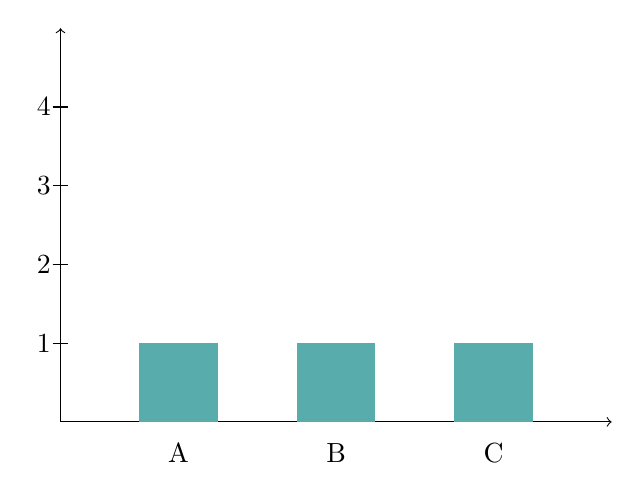
\begin{tikzpicture}
\draw[->] (0,0)--(7,0);\draw[->] (0,0)--(0,5);
\fill[teal!65] (1,0) rectangle (2,\SampleA);
\fill[teal!65] (3,0) rectangle (4,\SampleB);
\fill[teal!65] (5,0) rectangle (6,\SampleC);
\node at (1.5,-.4) {\lr{A}};\node at (3.5,-.4) {\lr{B}};\node at (5.5,-.4) {\lr{C}};
\foreach \y in {1,2,3,4} {\draw (-.1,\y)--(.1,\y);\node[left] at (0,\y) {\lr{\y}};}
\end{tikzpicture}

\caption[مقایسه ساختگی]{مقایسه سه مقدار ساختگی از پوشه داده‌های نمونه؛ از این نمودار نباید نتیجه پژوهشی گرفت.}\label{fig:chart}
\end{ThesisChart}
مقادیر از یک پرونده مشترک خوانده می‌شوند؛ با تغییر داده‌ها و ساخت دوباره، نمودار به‌روز می‌شود.

\chapter{بحث و جمع‌بندی}
این قالب نمونه‌ای از سازمان‌دهی یک متن دانشگاهی را فراهم می‌کند.
\section{محدودیت‌ها}
مثال‌ها برای نمایش قابلیت‌های حروف‌چینی هستند. محتوای علمی، منابع و انطباق با مقررات جاری باید توسط نویسنده بررسی شوند.
\section{کارهای آینده}
برای توسعه متن، یک پرونده فصل اضافه کنید و آن را در پرونده اصلی فراخوانی کنید. نمونه جدول چندصفحه‌ای در پیوست آمده است.


\clearpage
\phantomsection
\chapter*{منابع و مآخذ}
\addcontentsline{toc}{chapter}{منابع و مآخذ}
\begin{latin}\thesislatinfont\fontsize{10.5pt}{12pt}\selectfont
\renewcommand*{\bibfont}{\thesislatinfont\fontsize{10.5pt}{12pt}\selectfont}
\DeclareFieldFormat{labelnumberwidth}{%
  {\fontsize{9.5pt}{12pt}\selectfont[}#1{\fontsize{9.5pt}{12pt}\selectfont]}}
\setlength{\bibitemsep}{3pt}
\setlength{\bibparsep}{0pt}
\setlength{\biblabelsep}{0.6em}
\printbibliography[heading=none]
\end{latin}

% Appendices keep the main Arabic folio sequence but use Persian letters.
\clearpage
\appendix
% Only appendix titles appear in the main contents.
\addtocontents{toc}{\protect\setcounter{tocdepth}{0}}
\renewcommand{\thechapter}{\thesisappendixletter{\value{chapter}}}
\renewcommand{\thesischapterprefix}{پیوست}
\chapter{مثال‌های تکمیلی}
\section{جدول بلند}
\begin{longtable}{rr}
\caption[نمونه جدول بلند]{نمونه ساختار جدول بلند با سربرگ تکرارشونده.}\label{tab:long}\\
\toprule شماره & توضیح\\\midrule\endfirsthead
\toprule شماره & توضیح\\\midrule\endhead
\bottomrule\endfoot
\thesisnum{۱} & ردیف نمونه برای نمایش ادامه جدول\\
\thesisnum{۲} & ردیف نمونه برای نمایش ادامه جدول\\
\thesisnum{۳} & ردیف نمونه برای نمایش ادامه جدول\\
\thesisnum{۴} & ردیف نمونه برای نمایش ادامه جدول\\
\thesisnum{۵} & ردیف نمونه برای نمایش ادامه جدول\\
\thesisnum{۶} & ردیف نمونه برای نمایش ادامه جدول\\
\thesisnum{۷} & ردیف نمونه برای نمایش ادامه جدول\\
\thesisnum{۸} & ردیف نمونه برای نمایش ادامه جدول\\
\thesisnum{۹} & ردیف نمونه برای نمایش ادامه جدول\\
\thesisnum{۱۰} & ردیف نمونه برای نمایش ادامه جدول\\
\thesisnum{۱۱} & ردیف نمونه برای نمایش ادامه جدول\\
\thesisnum{۱۲} & ردیف نمونه برای نمایش ادامه جدول\\
\thesisnum{۱۳} & ردیف نمونه برای نمایش ادامه جدول\\
\thesisnum{۱۴} & ردیف نمونه برای نمایش ادامه جدول\\
\thesisnum{۱۵} & ردیف نمونه برای نمایش ادامه جدول\\
\thesisnum{۱۶} & ردیف نمونه برای نمایش ادامه جدول\\
\thesisnum{۱۷} & ردیف نمونه برای نمایش ادامه جدول\\
\thesisnum{۱۸} & ردیف نمونه برای نمایش ادامه جدول\\
\thesisnum{۱۹} & ردیف نمونه برای نمایش ادامه جدول\\
\thesisnum{۲۰} & ردیف نمونه برای نمایش ادامه جدول\\
\thesisnum{۲۱} & ردیف نمونه برای نمایش ادامه جدول\\
\thesisnum{۲۲} & ردیف نمونه برای نمایش ادامه جدول\\
\thesisnum{۲۳} & ردیف نمونه برای نمایش ادامه جدول\\
\thesisnum{۲۴} & ردیف نمونه برای نمایش ادامه جدول\\
\thesisnum{۲۵} & ردیف نمونه برای نمایش ادامه جدول\\
\thesisnum{۲۶} & ردیف نمونه برای نمایش ادامه جدول\\
\thesisnum{۲۷} & ردیف نمونه برای نمایش ادامه جدول\\
\thesisnum{۲۸} & ردیف نمونه برای نمایش ادامه جدول\\
\thesisnum{۲۹} & ردیف نمونه برای نمایش ادامه جدول\\
\thesisnum{۳۰} & ردیف نمونه برای نمایش ادامه جدول\\
\thesisnum{۳۱} & ردیف نمونه برای نمایش ادامه جدول\\
\thesisnum{۳۲} & ردیف نمونه برای نمایش ادامه جدول\\
\end{longtable}
\begin{ThesisLandscape}
\section{صفحه افقی}
این صفحه برای جدول‌ها و شکل‌های عریض مناسب است.
\begin{table}[ht]\centering
\caption[جدول افقی]{یک جدول نمونه در صفحه افقی.}
\begin{tabular}{rrrr}\toprule روش & ورودی & پردازش & خروجی\\\midrule
نمونه & متن & بررسی & گزارش\\\bottomrule\end{tabular}
\end{table}
\end{ThesisLandscape}

\addtocontents{toc}{\protect\setcounter{tocdepth}{2}}

% Persian semantic entries remain active for \gls first-use forms, while only
% the used English-to-Persian registry is printed at the end.
\clearpage
\printnoidxglossary[type=enfa,title={واژه‌نامه انگلیسی به فارسی},style=thesisenfa,sort=standard]

\ifThesisIncludeEnglishPages
  \clearpage
  \pagestyle{empty}\pagenumbering{gobble}
  \ThesisEnglishAbstractPage
  \ThesisEnglishTitlePage
\fi

\end{document}
